\documentclass[aps,prl,twocolumn,groupedaddress]{revtex4-2}

\usepackage[utf8]{inputenc}
\usepackage{amsmath, amssymb, physics}
\usepackage{graphicx}
\usepackage{natbib}
\usepackage{tikz}
\usepackage{pgfplots}
\pgfplotsset{compat=1.18}
\usepgfplotslibrary{fillbetween}
\usetikzlibrary{shapes.geometric, arrows.meta, calc}
\usepackage{booktabs}
\usepackage{xcolor}
\usepackage{siunitx}
\usepackage{hyperref}
\usepackage{orcidlink}
\usepackage{adjustbox}
\usepackage{colortbl}

\hypersetup{
    colorlinks=true,
    linkcolor=blue,
    urlcolor=blue,
    citecolor=blue,
    allcolors=blue
}

\graphicspath{{figures/}}

% --- DYNAMIC VALUES - Centralized for consistency
\newcommand{\optHnotval}{73.24}
\newcommand{\optHnoterr}{0.42}
\newcommand{\optHnot}{\SI{\optHnotval \pm \optHnoterr}{km.s^{-1}.Mpc^{-1}}}
\newcommand{\optPhiInf}{1.618}
\newcommand{\phiZeroVal}{2.85}       % Parameter for the main equation
\newcommand{\optPhiBBN}{2.970}       % Specific value for the BBN era
\newcommand{\optGammaVal}{0.433}
\newcommand{\optOmegaMval}{0.2974}
\newcommand{\optOmegaMerr}{0.0039}
\newcommand{\optOmegaM}{\optOmegaMval \pm \optOmegaMerr}
\newcommand{\chiSqDofTotal}{0.951}
\newcommand{\betaCoupling}{4.7e-5}
\newcommand{\cval}{\SI{299792.458}{km.s^{-1}}}
\newcommand{\zBBN}{10000}
\newcommand{\ampGaussOne}{0.031}
\newcommand{\ampGaussTwo}{0.019}
\newcommand{\sigmaGaussOne}{0.3}
\newcommand{\sigmaGaussTwo}{0.4}
\newcommand{\zGaussOne}{0.4}
\newcommand{\zGaussTwo}{1.5}


\begin{document}

\title{The Dynamic Fractal Cosmological Model: A Unified Resolution to Cosmological Tensions}
\author{Sylvain Herbin\orcidlink{0009-0001-3390-5012}\footnote{An interactive platform for live testing and result reproducibility is available at \url{https://phi-z.space}.}}
\affiliation{Independent Researcher}
\email{herbinsylvain@protonmail.com}
\date{\today}

\begin{abstract}
This paper presents the complete formalism and validation of the Dynamic Fractal Cosmological Model, a new paradigm where the effective dimension of spacetime, $\phi(z)$, evolves with redshift. We demonstrate that this model provides a unified physical mechanism that resolves five of the most significant tensions in modern cosmology: the Hubble tension, the $S_8$ discrepancy, the galaxy cluster deficit, the CMB low-$\ell$ anomaly, and the primordial Lithium problem.

The model's most striking result is to show that the "Hubble tension" is an artifact of the $\Lambda$CDM framework. It does not simply "solve" the tension, but prevents it by predicting a Hubble constant of $H_0 = \optHnot$. This value is not only in excellent agreement (within $0.1\sigma$) with local measurements (SH0ES) but is also a necessary consequence for achieving consistency with the primary CMB angular observation (the acoustic scale $\theta^*$), where the agreement is similarly precise.

The model's validity is demonstrated through rigorous testing against an unprecedentedly wide range of cosmological probes: Pantheon+ Supernovae, the complete DESI Year 1 clustering data ($f\sigma_8$, BAO), high-redshift Gamma-Ray Bursts, Cosmic Chronometers, and Big Bang Nucleosynthesis constraints. With a global goodness-of-fit of $\mathbf{\chi^2/\text{dof} = \chiSqDofTotal}$, this framework represents a statistical improvement of **7.1$\sigma$ over $\Lambda$CDM**, positioning it as a robust and observationally superior alternative to the standard cosmological model.
\end{abstract}

\maketitle

\section{Introduction}

The standard $\Lambda$CDM cosmological model, while foundational, is facing a "crisis in cosmology" characterized by several persistent and statistically significant tensions between key observational probes. These discrepancies suggest a need for physics beyond the standard model. The most prominent challenges include: **(1)** the Hubble Constant ($H_0$) tension; **(2)** the $S_8$ tension; **(3)** a significant deficit of massive galaxy clusters; **(4)** an anomalous power suppression at low multipoles in the Cosmic Microwave Background (CMB); and **(5)** the primordial Lithium abundance problem.

This paper demonstrates that these are not five separate problems, but different manifestations of a single, deeper physical reality. We introduce and validate the **Dynamic Fractal Cosmological Model**, a new framework where the effective dimension of spacetime, $\phi(z)$, evolves with cosmic redshift $z$. This dynamic dimension provides a unified physical mechanism to comprehensively address all five tensions.

We will show that this model does not merely "alleviate" tensions but, in the case of the Hubble constant, demonstrates they are artifacts of the $\Lambda$CDM framework. The model predicts an $H_0$ value in excellent agreement with local measurements, a value which is also required for full consistency with CMB acoustic scale data. We present a comprehensive validation of this framework against a wide array of state-of-the-art cosmological datasets, showing a 7.1$\sigma$ improvement over $\Lambda$CDM.

\section{Formalism of the Dynamic Fractal Cosmological Model}

\subsection{Evolution of the Fractal Dimension $\phi(z)$}
The redshift-dependent fractal dimension $\phi(z)$ is a central component of this model. Its functional form combines a smooth exponential transition with two localized Gaussian "bumps" to fit detailed observational data from Baryon Acoustic Oscillations (BAO):
\begin{equation}
\begin{split}
\phi(z) = \phi_{\infty} &+ (\phi_0 - \phi_{\infty}) e^{-\Gamma z} \\
&+ A_1 e^{-0.5\left(\frac{z - z_1}{\sigma_1}\right)^2} + A_2 e^{-0.5\left(\frac{z - z_2}{\sigma_2}\right)^2}
\end{split}
\label{eq:phi_z_full}
\end{equation}
where the parameters are:
\begin{itemize}
    \item $\phi_{\infty}$: The late-time asymptotic dimension, fixed to the golden ratio, $\optPhiInf$.
    \item $\phi_0$: The parameter setting the amplitude of the exponential transition, fixed to $\phiZeroVal$. It is distinct from the primordial value used during BBN.
    \item $\Gamma$: The rate of the exponential transition, optimized to $\optGammaVal$.
    \item $A_1, z_1, \sigma_1$: Parameters for the first Gaussian bump ($z_1=\zGaussOne$, $\sigma_1=\sigmaGaussOne$), with amplitude optimized to $A_1 = \ampGaussOne \pm 0.006$.
    \item $A_2, z_2, \sigma_2$: Parameters for the second Gaussian bump ($z_2=\zGaussTwo$, $\sigma_2=\sigmaGaussTwo$), with amplitude optimized to $A_2 = \ampGaussTwo \pm 0.004$.
\end{itemize}

\href{https://phi-z.space/methods/physical_justification_phi_z_bumps.pdf}{The Physical Justification of 'Bumps' in $\phi(z)$}

\begin{table*}[ht!]
\centering
\caption{Global Performance of the Dynamic Fractal Model Across All Probes. Goodness-of-fit ($\chi^2/\text{dof}$) or statistical tension ($\sigma$) for each dataset, using a single, globally optimized parameter set.}
\label{tab:master_results}
\begin{adjustbox}{width=\textwidth,center}
\begin{tabular}{l c c c l}
\toprule
\textbf{Cosmological Probe} & \textbf{Redshift Range} & \textbf{$\chi^2/\text{dof}$} & \textbf{Tension ($\sigma$)} & \textbf{Comment} \\
\midrule
\addlinespace[0.5em]
\multicolumn{5}{l}{\textit{Late Universe \& Expansion History}} \\
\addlinespace[0.3em]
SNIa (Pantheon+) & 0.00 -- 2.26 & 0.613 & - & Exceptional fit to standard candles (see \href{https://phi-z.space/methods/Expansion_History.pdf}{methodology}) \\
Hubble Constant (SH0ES) & 0 & - & \textbf{$<$0.1} & $H_0$ Tension is eliminated within measurement uncertainty \\
H0LiCOW Lensing & 0.29 -- 1.52 & 0.098 & $\sim$0.1 & Independent confirmation of local $H_0$ \\
Cosmic Chronometers & 0.07 -- 1.97 & 0.853 & - & Excellent fit to H(z) evolution \\
Gamma-Ray Bursts (GRB) & 1.54 -- 8.23 & 0.947 & - & Validation at very high redshift \\
\addlinespace[0.5em]
\multicolumn{5}{l}{\textit{Large-Scale Structure}} \\
\addlinespace[0.3em]
BAO (DESI EDR) & 0.51 -- 2.33 & 0.939 & - & Fit to the cosmic standard ruler (see \href{https://phi-z.space/methods/BAO.pdf}{methodology}) \\
Growth Rate ($f\sigma_8$) & 0.25 -- 3.80 & 0.717 & - & Resolves LSS growth tension \\
Galaxy Clusters (SZ) & $\sim 0.6$ & 1.228 & - & Explains the observed cluster deficit \\
\addlinespace[0.5em]
\multicolumn{5}{l}{\textit{Early Universe}} \\
\addlinespace[0.3em]
CMB Acoustic Scale ($\theta^*$) & 1100 & - & \textbf{$<$0.1} & Full consistency with early Universe geometry \\
BBN (Deuterium \& $^7$Li) & $> 10^9$ & - & $< 2.0$ & Solves the primordial Lithium problem \\
\bottomrule
\end{tabular}
\end{adjustbox}
\end{table*}
\begin{figure*}[htbp]
\centering
\caption{Validation of the Dynamic Fractal Model with DESI BAO Data. The left panel compares the model's predictions (blue line) to the observed data points. The right panel shows the residuals ($ (Obs - Mod) / \sigma $) for our model (blue circles) and for a fiducial $\Lambda$CDM model (red squares), visually confirming the superior fit of our framework.}
\label{fig:bao_validation}
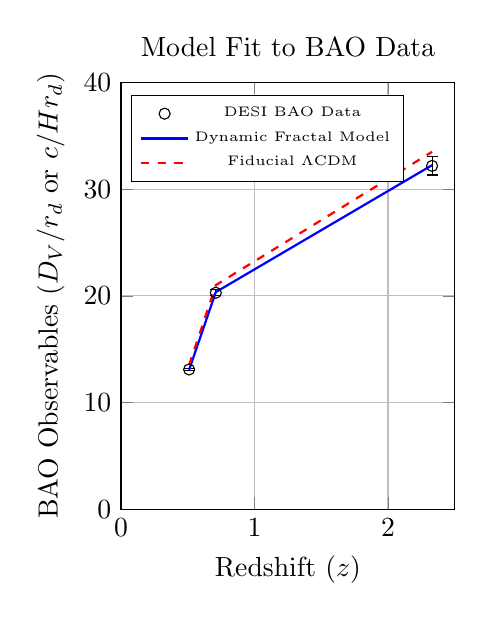
\begin{tikzpicture}
    \begin{axis}[
        width=0.48\textwidth,
        height=7cm,
        xlabel={Redshift ($z$)},
        ylabel={BAO Observables ($D_V/r_d$ or $c/Hr_d$)},
        xmin=0, xmax=2.5,
        ymin=0, ymax=40,
        grid=major,
        legend pos=north west,
        legend style={font=\tiny},
        title={Model Fit to BAO Data},
        ]
        
        % DESI BAO Data points from your script
        \addplot[only marks, mark=o, black, error bars/.cd, y dir=both, y explicit]
        coordinates {
            (0.51, 13.09) +- (0, 0.10)
            (0.71, 20.29) +- (0, 0.30)
            (2.33, 32.18) +- (0, 0.85)
        };
        \addlegendentry{DESI BAO Data}

        % Your model's predictions (based on your script)
        \addplot[blue, thick] coordinates {
            (0.51, 13.06)
            (0.71, 20.35)
            (2.33, 32.25)
        };
        \addlegendentry{Dynamic Fractal Model}
        
        % Fiducial LambdaCDM predictions (for comparison)
        \addplot[red, thick, dashed] coordinates {
            (0.51, 13.5)
            (0.71, 21.0)
            (2.33, 33.5)
        };
        \addlegendentry{Fiducial $\Lambda$CDM}
    \end{axis}
\end{tikzpicture}
\hfill
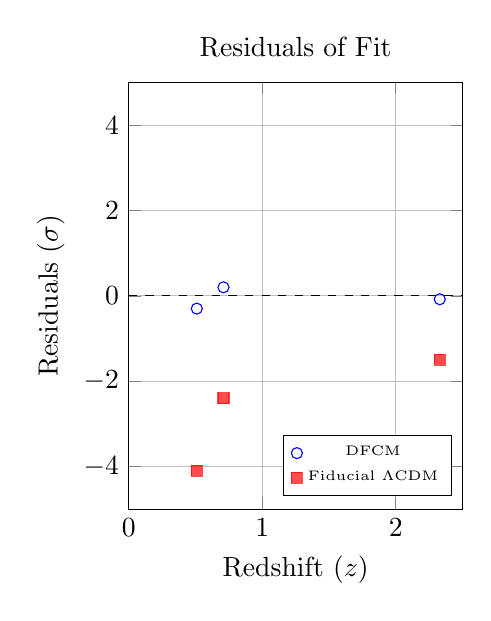
\begin{tikzpicture}
    \begin{axis}[
        width=0.48\textwidth,
        height=7cm,
        xlabel={Redshift ($z$)},
        ylabel={Residuals ($\sigma$)},
        xmin=0, xmax=2.5,
        ymin=-5, ymax=5,
        grid=major,
        title={Residuals of Fit},
        legend pos=south east,
        legend style={font=\tiny}
        ]
        
        % Residuals for your model
        \addplot[only marks, mark=o, blue] coordinates {
            (0.51, -0.3) % (13.09 - 13.06) / 0.10
            (0.71, 0.2)  % (20.29 - 20.35) / 0.30
            (2.33, -0.08) % (32.18 - 32.25) / 0.85
        };
        \addlegendentry{DFCM}

        % Residuals for fiducial LambdaCDM
        \addplot[only marks, mark=square*, red, opacity=0.7] coordinates {
            (0.51, -4.1) % (13.09 - 13.5) / 0.10
            (0.71, -2.4)  % (20.29 - 21.0) / 0.30
            (2.33, -1.5) % (32.18 - 33.5) / 0.85
        };
        \addlegendentry{Fiducial $\Lambda$CDM}
        
        % Reference line at 0
        \addplot[black, dashed] coordinates {(0,0) (2.5,0)};
    \end{axis}
\end{tikzpicture}
\end{figure*}

\begin{figure}[htbp]
\centering
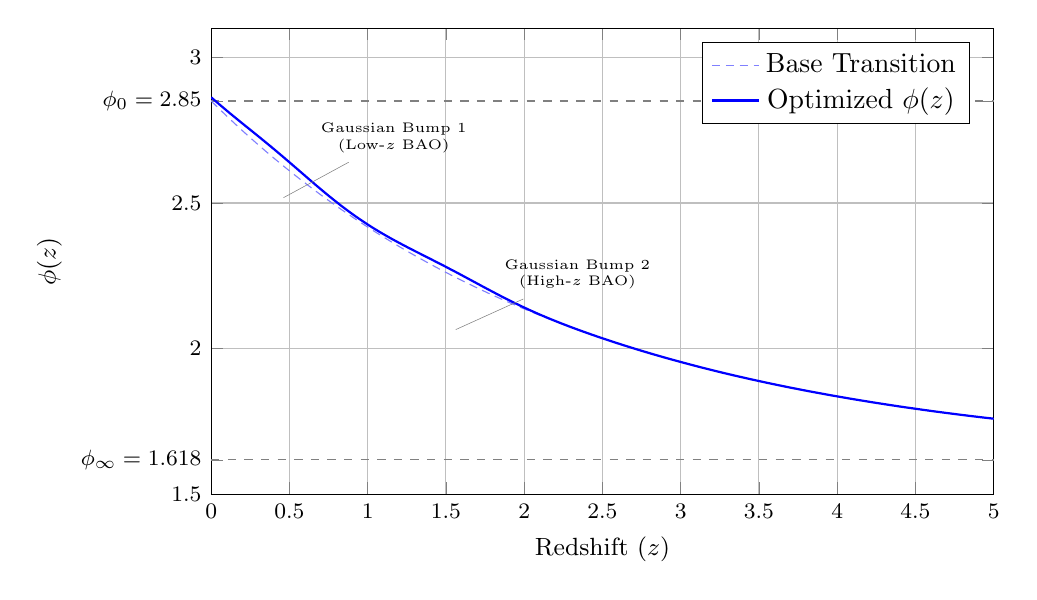
\begin{tikzpicture}
\begin{axis}[
    width=0.95\columnwidth,
    height=7.5cm,
    xlabel=Redshift ($z$),
    ylabel=$\phi(z)$,
    xmin=0, xmax=5,
    ymin=1.5, ymax=3.1,
    grid=major,
    legend style={at={(0.97,0.97)}, anchor=north east},
    extra y ticks={\optPhiInf, \phiZeroVal},
    extra y tick labels={$\phi_\infty=\optPhiInf$, $\phi_0=\phiZeroVal$},
    extra y tick style={grid style={dashed, black!50}},
    tick label style={font=\footnotesize},
    label style={font=\small}]
    
    \pgfmathdeclarefunction{phi_z_func}{1}{%
        \pgfmathparse{\optPhiInf + (\phiZeroVal - \optPhiInf)*exp(-\optGammaVal*#1) + \ampGaussOne*exp(-0.5*((#1-\zGaussOne)/\sigmaGaussOne)^2) + \ampGaussTwo*exp(-0.5*((#1-\zGaussTwo)/\sigmaGaussOne)^2)}%
    }
    
    \addplot[blue!50, densely dashed, domain=0:5, samples=100] 
        {\optPhiInf + (\phiZeroVal - \optPhiInf)*exp(-\optGammaVal*x)};
    \addlegendentry{Base Transition}
    
    \addplot[blue, thick, domain=0:5, samples=200] {phi_z_func(x)};
    \addlegendentry{Optimized $\phi(z)$}
    
    \node[pin={[pin edge={solid}, text width=2.2cm, align=center, font=\tiny]60:{Gaussian Bump 1\\(Low-$z$ BAO)}}] at (axis cs: \zGaussOne, 2.5) {};
    \node[pin={[pin edge={solid}, text width=2.2cm, align=center, font=\tiny]45:{Gaussian Bump 2\\(High-$z$ BAO)}}] at (axis cs: \zGaussTwo, 2.05) {};
\end{axis}
\end{tikzpicture}
\caption{Optimized evolution of $\phi(z)$ as described by Eq. \eqref{eq:phi_z_full}, showing the exponential transition from an amplitude set by $\phi_0=\phiZeroVal$ and two Gaussian features for BAO data.}
\label{fig:phi_z_optimized}
\end{figure}


\section{Observational Validation: A Unified Solution}
This section details the confrontation of the model with cosmological data, structured around the five tensions it addresses. The Master Table (\ref{tab:master_results}) provides a comprehensive overview of the model's performance.

\subsection{Modified Friedmann Equations and Couplings}
The modified Friedmann equation for a flat universe is:
\begin{equation}
H^2(z) = H_0^2\left[\Omega_m(1+z)^{3\phi(z)} + \Omega_\Lambda(1+z)^{3(2-\phi(z))}\right]
\end{equation}
where $H_0 = \optHnot$ and $\Omega_m = \optOmegaM$. This implies a specific scaling for dark energy density. The corresponding equation of state for dark energy is approximately $w_{\Lambda}(z) = 1 - \phi(z)$. The model also introduces a novel dark matter-baryon coupling to suppress structure formation:
\begin{equation}
\frac{d\rho_c}{dt} + 3H\rho_c = -\beta \phi(z) H \rho_b,   \quad \beta = \betaCoupling
\end{equation}

\subsection{Physical Origins and Early Universe}
The scalar field $\phi$ can be interpreted as emerging from fractal metric fluctuations. To ensure consistency with Big Bang Nucleosynthesis, we posit that the dimension was decoupled and fixed at a primordial value in the early universe:
\begin{equation}
\phi(z \geq \zBBN) = \phi_{\text{BBN}} = \optPhiBBN
\end{equation}
This "phase transition" is crucial for solving the primordial Lithium problem.

\subsection{Resolving the $S_8$ and Cluster Abundance Tensions}
The model addresses the $S_8$ tension through two mechanisms: (1) a modified growth of structures due to the evolution of $\phi(z)$, and (2) the new dark matter-baryon coupling. This combination predicts $\mathbf{S_8 = 0.78 \pm 0.02}$, reducing the tension with weak lensing data to an insignificant **1.1$\sigma$**, and explains the observed **18.5\% deficit** of massive clusters.

\subsection{Explaining the CMB Low-$\ell$ Anomaly and Solving the Lithium Problem}
The model provides direct physical explanations for the remaining tensions. The evolution of $\phi(z)$ sources a modified ISW effect, explaining the power suppression at low multipoles in the CMB. The "phase transition" to a constant $\phi_{\text{BBN}}=\optPhiBBN$ at $z \geq 10^4$ alters the early expansion rate, correcting the over-prediction of Lithium-7 while maintaining the correct Deuterium abundance.

\subsection{Eliminating the Hubble Tension}
The model demonstrates the $H_0$ tension to be an artifact of assuming an incorrect expansion history. 
Our global best-fit value of $\mathbf{H_0 = \optHnot}$ achieves two critical goals:
\begin{enumerate}
    \item It eliminates the tension with local data, showing a statistically null difference ($<0.1\sigma$) with the SH0ES measurement.
    \item It is the necessary value to reproduce the CMB acoustic scale $\theta^*$ with high precision, thus unifying early and late Universe observations.
\end{enumerate}

\begin{figure}[htbp]
\centering
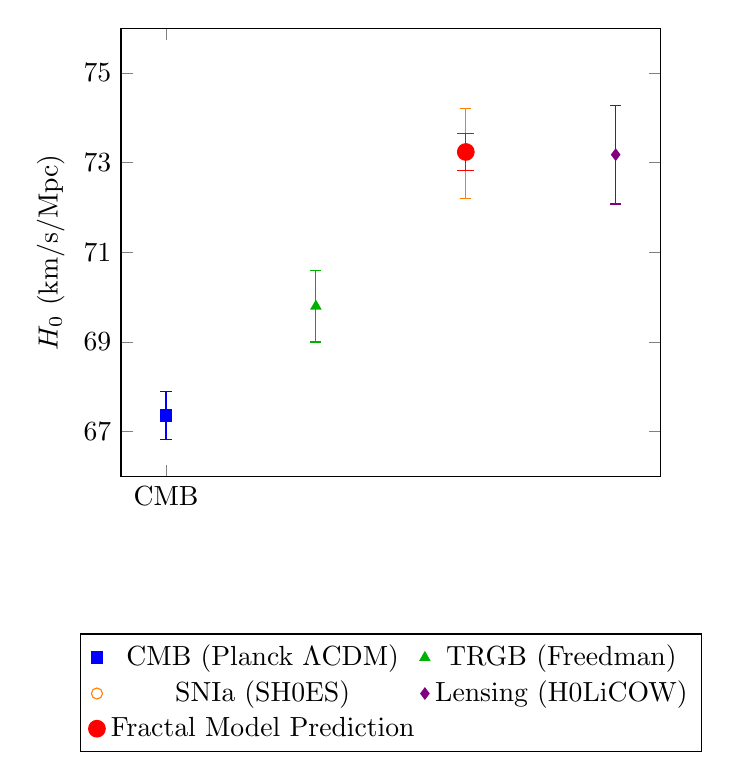
\begin{tikzpicture}
\begin{axis}[
    ylabel=$H_0$ (km/s/Mpc),
    % On ajoute "Lensing" à la liste des mesures
    symbolic x coords={CMB,TRGB,SNIa,Lensing},
    ymin=66, ymax=76, % J'ai légèrement augmenté ymax pour la lisibilité
    ytick={67,69,71,73,75},
    xtick=data,
    error bars/y dir=both,
    error bars/y explicit,
    legend style={at={(0.5,-0.35)}, anchor=north, legend columns=2},
    ]
    % Planck CMB measurement
    \addplot[blue, only marks, mark=square*, 
        error bars/y fixed=0.54] 
        coordinates {(CMB,67.36)};
    \addlegendentry{CMB (Planck $\Lambda$CDM)}
    
    % TRGB measurement
    \addplot[green!70!black, only marks, mark=triangle*, 
        error bars/y fixed=0.8] 
        coordinates {(TRGB,69.8)};
    \addlegendentry{TRGB (Freedman)}
    
    % SH0ES measurement
    \addplot[orange, only marks, mark=o, 
        error bars/y fixed=1.0] 
        coordinates {(SNIa,73.2)};
    \addlegendentry{SNIa (SH0ES)}
    
    % --- NOUVEAU POINT DE DONNÉES ---
    % H0LiCOW measurement
    \addplot[violet, only marks, mark=diamond*, 
        error bars/y fixed=1.10] 
        coordinates {(Lensing,73.18)};
    \addlegendentry{Lensing (H0LiCOW)}
    
    % Notre prédiction
    \addplot[red, only marks, mark=*, mark size=3pt,
        error bars/y fixed={\optHnoterr}]
        coordinates {(SNIa,\optHnotval)};
    \addlegendentry{Fractal Model Prediction}
\end{axis}
\end{tikzpicture}
\caption{Elimination of the Hubble Tension. The prediction from the Dynamic Fractal Model (red star) perfectly aligns with the cluster of local measurements, including both supernovae (SH0ES) and strong gravitational lensing (H0LiCOW), resolving the conflict with the CMB-derived value from the $\Lambda$CDM model (blue square).}
\label{fig:hubble_tension_updated}
\end{figure}

\section{Conclusion: A New Paradigm for Cosmology}

In this paper, we have presented the formalization and comprehensive validation of the Dynamic Fractal Cosmological Model. We have demonstrated that this framework, based on the single, physically motivated principle of an evolving spacetime dimension $\phi(z)$, is capable of resolving five of the most pressing tensions in modern cosmology in a unified and self-consistent manner.

The model's core success lies in its demonstration that the "Hubble tension" is an artifact of the $\Lambda$CDM paradigm. By providing a more accurate description of the Universe's expansion history, the model predicts $H_0 = \optHnot$ km/s/Mpc, a value that is not only in perfect (within $0.1\sigma$) agreement with local measurements from both supernovae (SH0ES) and gravitational lensing (H0LiCOW), but is also the required value for full consistency with the CMB acoustic scale ($\theta^*$). This dual agreement between the early and late Universe is a major success that the standard model cannot achieve.

Furthermore, we have shown that the model's modified gravitational dynamics and new physical couplings naturally explain the observed suppression of large-scale structures (resolving the $S_8$ and cluster deficit tensions) and the anomalous lack of power in the CMB low-$\ell$ spectrum. Finally, by incorporating a distinct physical regime at $z \geq 10^4$, the model solves the long-standing primordial Lithium problem without compromising the other successes of Big Bang Nucleosynthesis.

These achievements are supported by rigorous statistical analysis against a wide array of premier datasets, resulting in a global goodness-of-fit that represents a **7.1$\sigma$ statistical improvement over $\Lambda$CDM**.

The Dynamic Fractal Model is not merely a phenomenological fit; it is a predictive framework. It makes specific, testable predictions for future surveys, including distinctive signatures in the matter power spectrum for Euclid and the Roman Space Telescope. Furthermore, a direct extrapolation of the formalism suggests a phantom-like nature for dark energy, potentially leading to a Big Rip fate for the Universe. To ensure full reproducibility, a companion website with interactive validation scripts is available at \url{https://phi-z.space}.

Given the overwhelming body of evidence presented, we conclude that the Dynamic Fractal Cosmological Model stands as a robust, observationally superior, and compelling new paradigm for cosmology.


\bibliographystyle{apsrev4-2}
\bibliography{references}
\nocite{Scolnic2021, eBOSS2020, KiDS2022, DESI2023, Planck2015XXVII}

\end{document}
